\documentclass[conference]{IEEEtran}
% -------------------- PACKAGES --------------------
\usepackage{cite}
\usepackage{amsmath,amssymb}
\usepackage{graphicx}
\usepackage{booktabs}
\usepackage{multirow}
\usepackage{array}
\usepackage{url}
\usepackage{float}
\renewcommand{\IEEEkeywordsname}{Keywords}
% -------------------- TITLE --------------------
\title{Hybrid AI-Based System for Student Performance and Placement Readiness Prediction}
% -------------------- AUTHORS --------------------
\author{
\IEEEauthorblockN{B Sanjeevaraya}
\IEEEauthorblockA{\textit{Dept. of CSE (AI\&ML)} \\
\textit{Vardhaman College of Engineering}\\
Hyderabad, India \\
sanjuspot789@gmail.com}
\and
\IEEEauthorblockN{B Sharath Chandra}
\IEEEauthorblockA{\textit{Dept. of CSE (AI\&ML)} \\
\textit{Vardhaman College of Engineering}\\
Hyderabad, India \\
sharathbandaari@gmail.com}
\and
\IEEEauthorblockN{J Pruthvi Raj}
\IEEEauthorblockA{\textit{Dept. of CSE (AI\&ML)} \\
\textit{Vardhaman College of Engineering}\\
Hyderabad, India \\
pruthvi71718@gmail.com}
\and
\IEEEauthorblockN{T. Ishverya}
\IEEEauthorblockA{\textit{Dept. of CSE (AI\&ML)} \\
\textit{Vardhaman College of Engineering}\\
Hyderabad, India \\
tontaishverya97@gmail.com}
\and
\IEEEauthorblockN{M. A. Jabbar}
\IEEEauthorblockA{\textit{Dept. of CSE (AI\&ML)} \\
\textit{Vardhaman College of Engineering}\\
Hyderabad, India \\
jabbar.meerja@gmail.com}
}
% -------------------- DOCUMENT --------------------
\begin{document}
\maketitle

% -------------------- ABSTRACT --------------------
\begin{abstract}
The grade sheets and attendance registers have been
the traditional ways of assessing student potential in
engineering colleges over the decades. But they have
failed to do so. Students who excel in placement drives
may not necessarily have the highest marks. Similarly,
students with perfect attendance records may not
necessarily be ready to take on industry. Something more complete is needed. This paper presents a hybrid deep learning system that pulls together 23 student attributes spanning four dimensions academic history, technical skills, career preparation, and behavioral indicators to simultaneously estimate an academic performance score and assign a placement readiness category of Low,Medium, or High. The core model pairs a Deep Neural Network handling static attribute inputs with an LSTM network reading semester score sequences, joining them at a fusion layer before dual-head output. The architecture was validated on 10,001 student records, achieving 97.4\% classification accuracy and an F1-score of 0.974  improvements of 9 and 11.6 percentage points over Random Forest and Decision Tree baselines. A weighted multi-task loss formulation, with classification weighted at 1.8 and regression at 0.35, was found to be a significant factor in reaching this performance level.

\end{abstract}

% -------------------- KEYWORDS --------------------
\begin{IEEEkeywords}
Placement drives, Deep Neural Network, LSTM, Hybrid Machine Learning, Educational Data Mining
\end{IEEEkeywords}

% -------------------- INTRODUCTION --------------------
\section{Introduction}

There is a disconnect in how most engineering institutions evaluate their students. The internal systems used by colleges attendance tracking, grade sheets, semester results capture a narrow slice of what actually matters. A placement officer walking into a campus drive is not just looking at marks. They want to know if the student can code, whether they have worked on real projects, whether they have done an internship, and whether they can hold a technical conversation under pressure. None of that information typically lives anywhere in the college's internal records.

This problem has been recognized in the research community.Traditional grade sheets and attendance registers have been the standard for measuring student potential in engineering colleges for several decades now, and yet, they continue to fail in doing so. Early research in student outcome prediction, such as Cortez and Silva in~\cite{R1}, revealed that data-driven models could be more effective than traditional methods in identifying potential students, but it was based solely on grades, demographics, and attendance. Subsequent research used behavioral information from Learning Management Systems~\cite{R2,R3} to improve student potential prediction, but this is limited to what a student is doing within a system, not what they are creating outside it.

The introduction of LSTM-based architectures to this domain opened up a new direction~\cite{R5,R6}. Treating semester scores as a time series rather than independent data points makes it possible to capture whether a student is trending upward or downward — information that a simple average completely loses. But even these sequential models rarely pair academic trend data with career-facing indicators to assess placement readiness~\cite{R7}.

The system described in this paper addresses both halves of the problem. A 23-feature input space covers academic records, technical skill development, career activity, and behavioral self-ratings. A hybrid architecture processes static features through a DNN branch and semester score sequences through an LSTM branch, with both merged at a fusion layer. Two prediction heads simultaneously produce an academic score and a placement readiness label. Evaluated on 10,001 records, the approach achieves 97.4\% accuracy — a meaningful improvement over both baselines~\cite{R9,R10}, and one that reflects the cumulative benefit of a wider feature lens and a temporally-aware model architecture.
The objectives of this work are as follows:
\begin{enumerate}
    \item To design a 23-feature input space covering academic, skill-based, career-oriented, and behavioral dimensions, going beyond the 3 to 5 academic variables that most existing systems use.
    \item To build a hybrid DNN-LSTM model where one branch processes static features and another processes semester scores as a time series, with both fused before prediction.
    \item To predict academic performance as a continuous score and placement readiness as Low, Medium, or High simultaneously from one model using a weighted multi-task loss.
    \item To deploy the system as a working web application with student and faculty portals, resume scanning, certificate OCR verification, and a job recommendation module.
    % \item To evaluate the model against properly tuned Decision Tree and Random Forest baselines using accuracy, precision, recall, F1-score, and RMSE on a held-out test set.
    \item To evaluate the model against properly tuned Decision
    Tree and Random Forest baselines using accuracy, precision,
    recall, F1-Score, and RMSE in a holdout test set.
\end{enumerate}

% The remainder of this paper is structured as follows: Section~\ref{sec:Literative survey} reviews related work. Section~\ref{sec:methodology} details the system design and model. Section~\ref{sec:results} reports experimental findings. Section~\ref{sec:conclusion} concludes with future directions.


The remainder of the paper is structured as follows:
Section II reviews related work. Section III details the design and model of the system. Section~\ref{sec:results} reports the experimental findings. Section~\ref{sec:conclusion} concludes with future directions.

% --------------------LITERATURE SURVEY --------------------

\section{Literature survey}
However, conventional parameters such as grades and attendance alone are not sufficient to measure the real potential of the student. Today, it is not just academics; it is the practical knowledge, internships, projects, and communication skills as well. 

In the earlier studies, it was seen how data-driven models could perform better than conventional models, but the data considered was only academic and demographic in nature. With the advent of Learning Management Systems, the behavioral data came into the picture, but the external factors such as internships and projects were not considered.

To overcome these limitations, advanced models like LSTM were introduced, which analyze student performance as a sequence over time rather than as isolated data points. This allows the system to understand trends, such as whether a student is improving or declining, which provides deeper insights than simple averages. Building on this idea, the proposed system uses a hybrid architecture that combines Deep Neural Networks and LSTM. 

Before feeding data into the model, several preprocessing steps are applied to ensure accuracy and consistency. These include normalization to balance feature importance, encoding techniques to handle categorical data, and sequence masking to manage incomplete semester records without introducing errors. The system also addresses class imbalance by assigning appropriate weights during training, ensuring fair predictions across different categories of students. The architecture consists of two parallel branches: the DNN processes static features to capture complex relationships, while the LSTM processes sequential academic data to identify performance trends.
\begin{table*}[t]
\caption{Comparative Summary of Related Work}
\label{tab:litreview}
\centering
\renewcommand{\arraystretch}{1.3}
\begin{tabular}{|p{0.08\textwidth}|p{0.18\textwidth}|c|c|p{0.25\textwidth}|}
\hline
Ref & Method & Sequential & Career Features & Limitation \\ \hline
\cite{R1} & DT, RF & No & No & Academic only \\ \hline
\cite{R8} & NB, DT & No & No & No behavioral \\ \hline
\cite{R2} & Ensemble & No & No & LMS dependent \\ \hline
\cite{R3} & WEKA & No & No & Academic only \\ \hline
\cite{R6} & LSTM & Yes & No & No career \\ \hline
\cite{R7} & ML & Yes & No & No behavior \\ \hline
\cite{R10} & ML & No & Partial & No sequence \\ \hline
\cite{R15} & Fusion & Yes & No & No deployment \\ \hline
Proposed & DNN+LSTM & Yes & Yes & -- \\ \hline
\end{tabular}
\end{table*}
% -------------------- RELATED WORK --------------------
\section{Related Work}
\label{sec:related}

Predicting how students will perform has been studied across multiple waves of methodology, each adding something the previous one lacked.

The earliest work treated it as a straightforward classification problem. Cortez and Silva~\cite{R1} built decision tree and random forest models on Portuguese secondary school data using study time, household background, and past academic failures as inputs. Their work was significant for demonstrating that such prediction was possible at all, but the feature set reflected the data that was available at the time — academic and demographic, nothing more. Bharadwaj and Pal~\cite{R8} followed a similar path with undergraduate data and made an observation that turned out to be broadly applicable: feature selection decisions had more impact on final accuracy than model selection decisions.

\begin{figure}
    \centering
    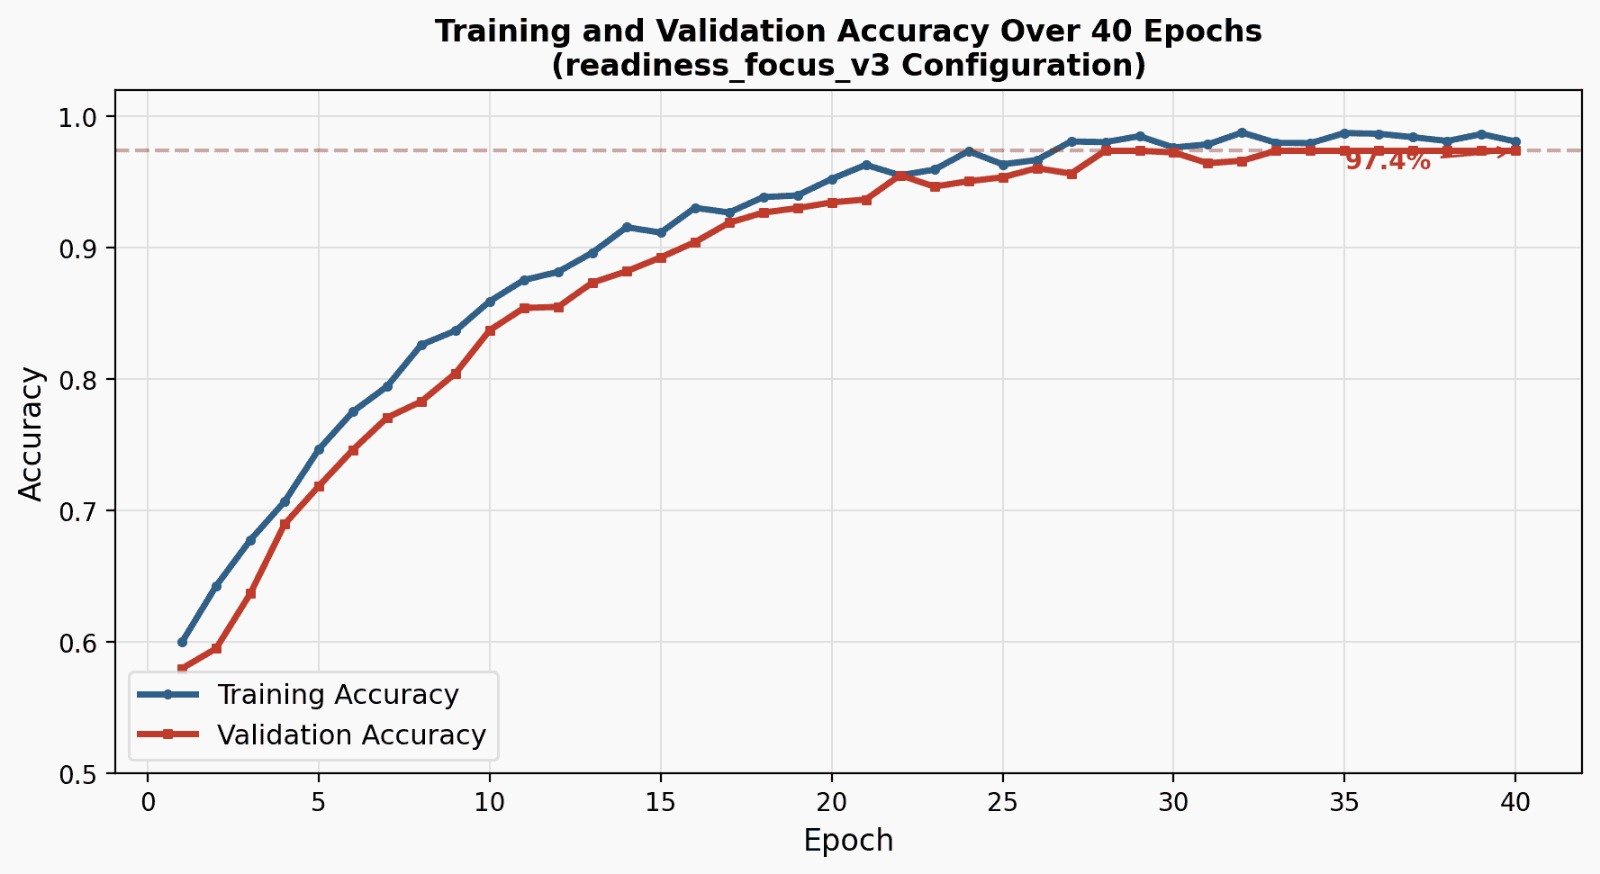
\includegraphics[width=0.8\linewidth]{Training.jpeg}
    \caption{Training and validation accuracy over 40 Epochs}
    \label{fig:placeholder}
\end{figure}

The universities are relying more on digital learning platforms. This means that we are swimming in new data from LMS records and so on. It’s all about behavior.This changed the way we think about dealing with sequences in models. Hochreiter and Schmidhuber designed this model to retain information over long periods. This is exactly like academic performance over a period of time rather than over an exam. Borges used this on LMS records. 

This completely changed our perspective on how to deal with a sequence in a model. This model was designed by Hochreiter and Schmidhuber to retain information for a long period of time. This is similar to academic performance over a long period of time, not over an exam. Borges used this on LMS records. This provided more accuracy than a traditional classifier. Xu has also shown that this is better than any model over a short period of time.Some people might overlook how those career features could fit, it feels like they get ignored too often.

\section{methodology}
\subsection{System Overview}

The proposed system has a layered structure that consists of a Streamlit-based interface for the front end, where students input their information and view the predictions. Then, there is a Python-based application that has the preprocessing steps, the parallel processing of the two models, and the fusion of the outputs before generating the two outputs simultaneously: a score for academic performance and a readiness score for placement.

The data that is entered by the students undergoes the preprocessing layer. After the preprocessing layer, the data goes through multiple paths based on the type of the feature. After passing through the parallel paths, the data goes through the fusion layer. Then the data goes through two different paths for the simultaneous generation of the results in the form of a score and a readiness classification.

The information of the students goes through the preprocessing steps and then is divided into two parallel paths based on the type of the feature. After passing through the parallel paths, the information goes through the fusion layer and then goes through two different paths for the simultaneous generation of the results in the form of a score and readiness classification. The faculty members can access the aggregated views of the readiness of the students using a different interface. Fig.~\ref{fig:architecture} illustrates the model architecture and data flow.

\begin{figure}
    \centering
    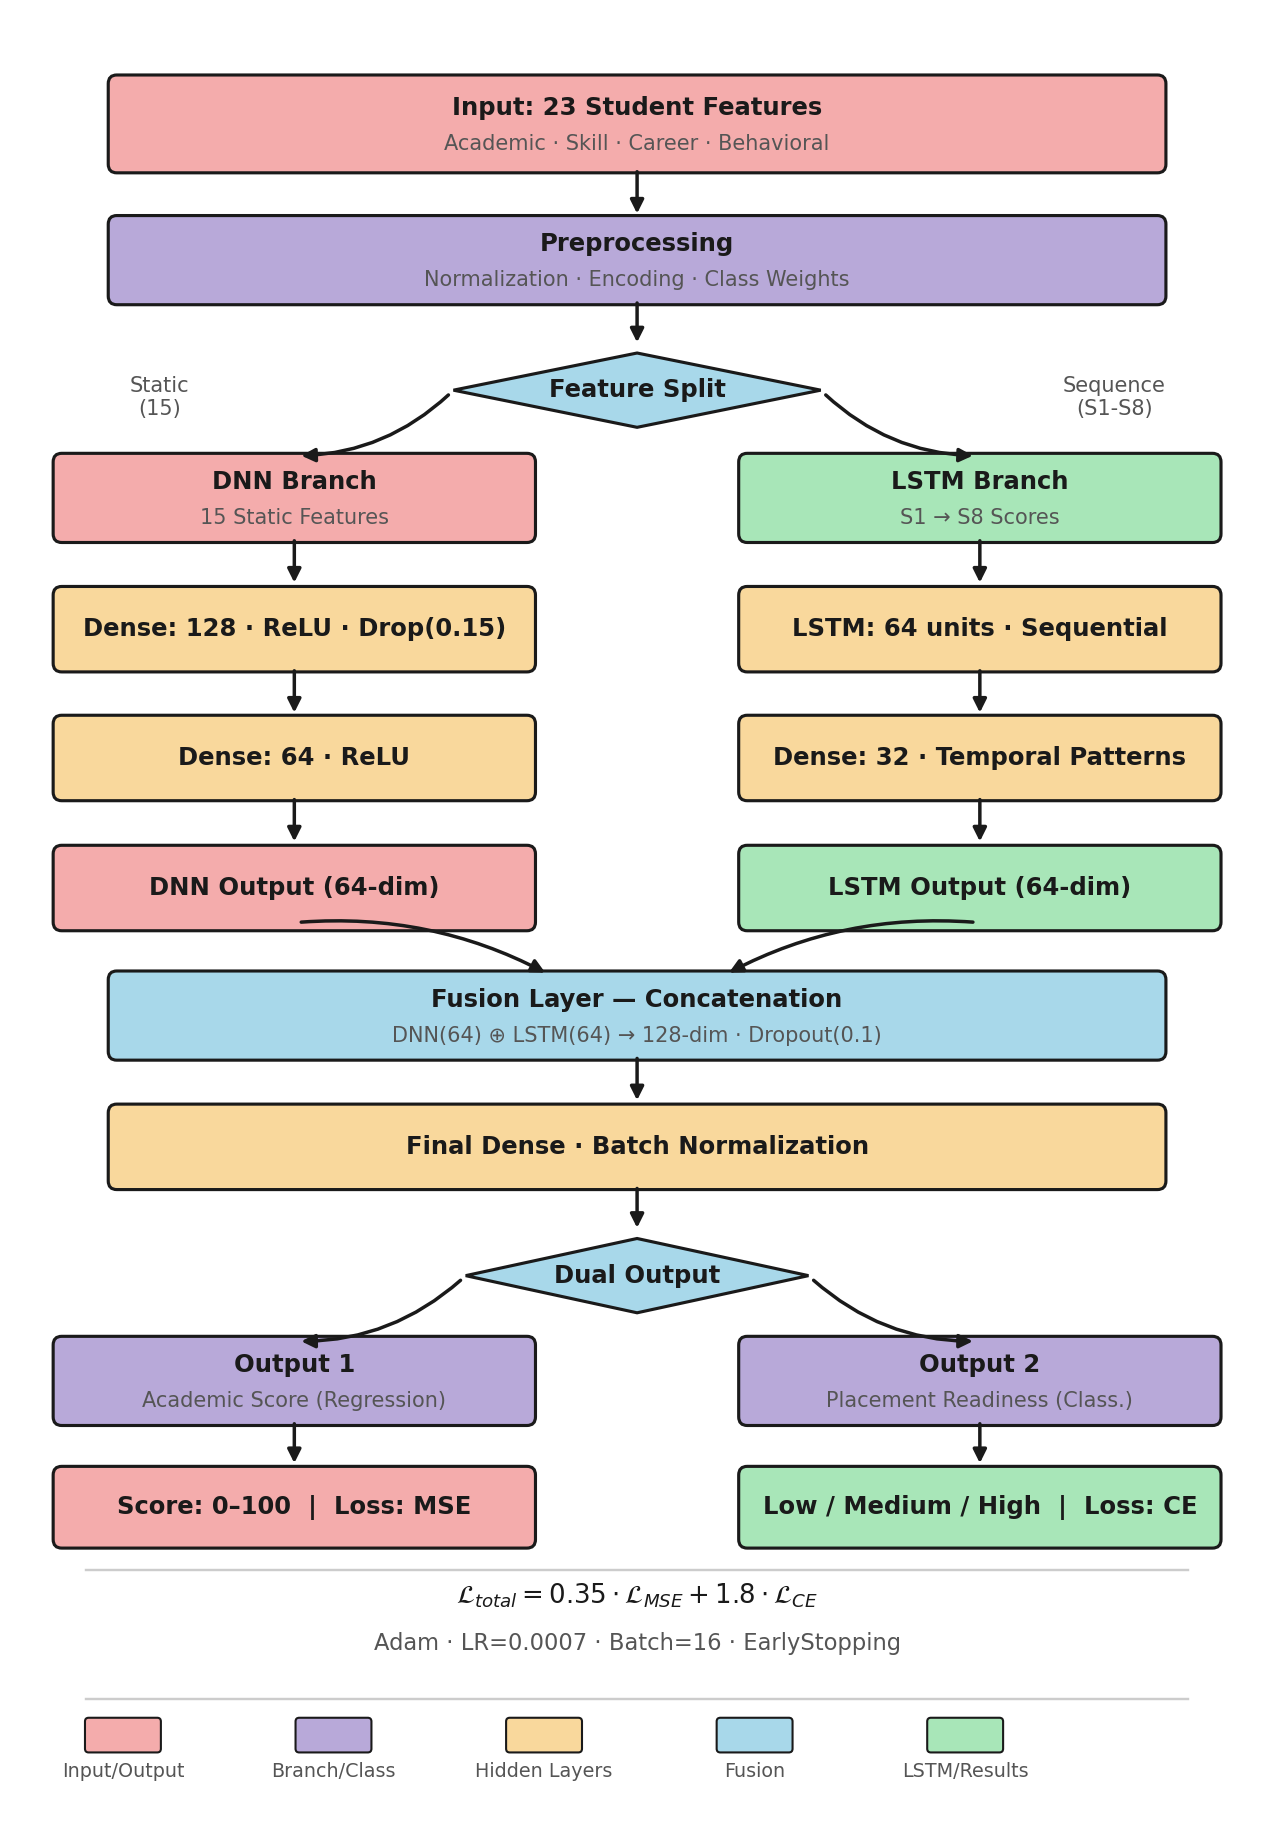
\includegraphics[width=\columnwidth]{model_architecture (1).png}
    \caption{Proposed Hybrid DNN-LSTM System Architecture}
    \label{fig:architecture}
\end{figure}

\subsection{Feature Engineering}

The input space has been extended beyond academia by incorporating relevant features. There are altogether 23 features, which fall under four categories as given in Table ~\ref{tab:features}. In the academic domain, S1 to S8, attendance percentage, backlogs, and year of study come under consideration. In the skills domain, features include skills learned, DSA language preference, hours spent coding per week, and how many coding profiles they currently have. In the careers domain, features include internship status, certifications, projects completed, domain of interest, and how many programming languages they know. In behavior, we look at how good they are at communicating, how much stress they face, and how much they are motivated, on a scale of 1-10.

\begin{table}
\caption{Feature Categories Used in the Proposed System}
\label{tab:features}
\centering
\renewcommand{\arraystretch}{1.3}
\begin{tabular}{|p{1.9cm}|p{5.6cm}|}
\hline
\textbf{Category} & \textbf{Features} \\
\hline
Academic & S1--S8 scores, attendance \%, backlogs, year of study \\
\hline
Skill-Based & Skills count, DSA language, coding hrs/week, coding profiles \\
\hline
Career-Oriented & Internships, certifications, projects, career domain, languages known \\
\hline
Behavioral & Communication, stress, motivation (1--10 each) \\
\hline
\end{tabular}
\end{table}

The semester score plays a two-fold role in this context: it contributes to the static academic feature vector, as well as being extracted as the ordered sequential input to the LSTM branch. Although the behavioral features are self-reported, their predictive weight has been demonstrated in combination with the objective academic data~\cite{R4}.

\subsection{Preprocessing Pipeline}

There are four preprocessing steps that are carried out before the data even enters the model. 

\textbf{Min-max normalization} This is done to prevent any one feature from dominating the input space based on its range:
\begin{equation}
x' = \frac{x - x_{\min}}{x_{\max} - x_{\min}}
\end{equation}

\textbf{One-hot encoding} is then carried out for the categorical input data – DSA language preference and the target career domain of the students. With this, the model can directly process this input.Lastly, sequence masking is carried out for those students who have not completed all eight semesters.

\textbf{Sequence masking} Deals with students who have not completed all eight semesters. In this case, instead of filling with zeros that might cause a wrong trend in the LSTM sequence, they are masked.

\textbf{Class weighting} addresses the natural skew in the readiness distribution (approximately 55\% High, 30\% Medium, 15\% Low). Weights of 8.63, 2.29, and 0.41 are assigned to Low, Medium, and High classes respectively during training, ensuring the model does not converge to a majority-class prediction bias.

\subsection{Model Architecture}

The proposed model has two parallel processing branches that operate independently before joining at a concatenation layer.

\textbf{DNN Branch:} Fifteen static features pass through two fully connected layers — 128 neurons with ReLU activation and 15\% dropout, followed by 64 neurons with ReLU. ReLU is used throughout the hidden layers because it avoids the saturation problems of sigmoid and tanh in deep networks and produces faster convergence on tabular input data. The branch output is a 64-dimensional representation vector.

\textbf{LSTM Branch:} Eight semester scores are processed as a time series by an LSTM layer with 64 hidden units, followed by a dense layer mapping to 64 dimensions. The LSTM cell update equations are:
\begin{equation}
f_t = \sigma(W_f \cdot [h_{t-1}, x_t] + b_f)
\end{equation}
\begin{equation}
i_t = \sigma(W_i \cdot [h_{t-1}, x_t] + b_i)
\end{equation}
\begin{equation}
o_t = \sigma(W_o \cdot [h_{t-1}, x_t] + b_o)
\end{equation}
\begin{equation}
C_t = f_t \odot C_{t-1} + i_t \odot \tanh(W_C \cdot [h_{t-1}, x_t] + b_C)
\end{equation}

where $f_t$, $i_t$, $o_t$ denote the forget, input, and output gates, and $C_t$ is the cell state at step $t$~\cite{R5}. Sigmoid gate activations constrain constrain their values to be in the range [0, 1] and act as differentiable switches
that control information retention and discarding.

\textbf{Fusion and Output:} The two 64-dimensional branch vectors are concatenated to create a 128-dimensional vector. After a 10\% dropout operation, this is passed through a final dense layer that simultaneously predicts two outputs: a continuous regression output for academic score (linear activation and MSE loss) and a three-class output for placement readiness (softmax activation and Cross-Entropy loss). The total training loss is:
\begin{equation}
\mathcal{L}_{total} = 0.35 \cdot \mathcal{L}_{MSE} + 1.8 \cdot \mathcal{L}_{CE}
\end{equation}

The relatively higher weight of the classification term is a reflection of the higher utility of this label in practice for students and faculty.

\subsection{Training Setup}

Three different models were tested with different weight ratios and learning rate strategies. The best-performing model had Adam as the optimizer with a learning rate of 0.0007 and a batch size of 16. It had a maximum of 40 epochs with the following callbacks: EarlyStopping with a patience of 10 and ReduceLROnPlateau.

% -------------------- RESULTS --------------------
\section{Results and Discussion}
\label{sec:results}

\subsection{Experimental Setup}

The dataset comprises 10,001 undergraduate engineering student records covering all 23 features. Data was split into 80\% training, 10\% validation, and 10\% test sets. The test partition was withheld entirely from all training and tuning decisions and used only for final evaluation. Both baseline models were tuned via grid search cross-validation: Decision Tree used entropy criterion with balanced class weights, Random Forest used 500 estimators at max depth 8 with balanced class weights.

\subsection{Performance Results}

Table~\ref{tab:results}indicates performance on test sets using all five evaluation metrics.


\begin{table}
\caption{Model Performance Comparison (Test Set, N = 10,001)}
\label{tab:results}
\centering
\renewcommand{\arraystretch}{1.3}
\begin{tabular}{|p{2.1cm}|p{0.8cm}|p{0.8cm}|p{0.85cm}|p{0.7cm}|p{0.75cm}|}
\hline
\textbf{Model} & \textbf{Acc.} & \textbf{Prec.} & \textbf{Recall} & \textbf{F1} & \textbf{RMSE} \\
\hline
Decision Tree & 85.8\% & 85.8\% & 85.8\% & 0.858 & 3.600 \\
\hline
Random Forest & 88.4\% & 90.4\% & 88.4\% & 0.891 & 2.463 \\
\hline
\textbf{Hybrid DNN+LSTM} & \textbf{97.4\%} & \textbf{97.4\%} & \textbf{97.4\%} & \textbf{0.974} & \textbf{1.200} \\
\hline
\end{tabular}
\end{table}

\subsection{Configuration Search}

Table~\ref{tab:configs} indicates validation readiness accuracy using all three configurations tested.

\begin{table}
\caption{Training Configuration Comparison}
\label{tab:configs}
\centering
\renewcommand{\arraystretch}{1.3}
\begin{tabular}{|p{2.9cm}|p{2cm}|p{1.4cm}|}
\hline
\textbf{Configuration} & \textbf{Val. Acc.} & \textbf{Epochs} \\
\hline
balanced\_v1 & 91.50\% & 30 \\
\hline
readiness\_focus\_v2 & 97.25\% & 31 \\
\hline
\textbf{readiness\_focus\_v3} & \textbf{97.44\%} & \textbf{40} \\
\hline
\end{tabular}
\end{table}

\subsection{Analysis}

Three points are evident from this data.

The LSTM contribution is not an artifact and is measurable. For tree-based models, semester scores are viewed as eight different input variables. There is no mechanism by which tree-based models can recognize trends. A student who improves from 55 to 77 over four semesters and one who decreases from 77 to 55 are indistinguishable to a random forest once scores are averaged or viewed as a vector. However, the LSTM recognizes these scores in a particular order and has different internal representations for each student's score series [6].

The new feature set also contributes independently of
the architecture. Internships, certifications, and motivations
contain information that is simply not present in academic
data sets. The improvement in accuracy over the baseline
models using the same academic data set validates that these
new dimensions are predictive, which is in line with the gaps
identified by Sghir et al. ~\cite{R4} and the results regarding
employability by Qiu et al. ~\cite{R10}.

The effectiveness of using a weighted loss was more
significant than initially anticipated. Changing from equal
weighting to 1.8 for classification and 0.35 for regression,
without any modifications to the architecture, data sets,
or optimizer, resulted in a 5.75-point increase in accuracy
between balanced v1 and readiness focus v3.
The relative weighting of task losses is a true
hyperparameter in multi-task learning and should be given
as much consideration as the number of layers and activation
functions.

In the context of the regression's performance, the RMSE of 1.20 on a 100-point scale implies that the average prediction made by the algorithm is one point away from the actual score. This is substantially better than the baseline's RMSEs of 3.60 and 2.46, which places it in the realm of early intervention in academic risk.~\cite{R7}.

% -------------------- CONCLUSION --------------------
\section{Conclusion}
\label{sec:conclusion}

This paper described a hybrid DNN-LSTM system for predicting student academic performance and placement readiness
from a 23-feature multi-dimensional input space. Two parallel
model branches — one for static profile features, one for
sequential semester scores — are fused before producing
simultaneous regression and classification outputs through a
weighted joint loss function.

On 10,001 student records, the model achieved 97.4\% accuracy and an F1-score of 0.974, with an RMSE of 1.20 on score
prediction. These results reflect the combined contribution of
a wider feature space, a temporally-aware architecture, and
deliberate loss weight calibration. None of these factors in
isolation produced comparable results — the improvement is
attributable to their combination.

The system is deployed as a functional web application.
Students receive placement readiness assessments and feature level feedback. Faculty gain a department-wide risk view.
Three auxiliary modules — PDF-based resume skill extraction, OCR-based certificate verification, and rule-based job
matching — extend the system beyond prediction into practical
career guidance.

Planned extensions include attention-weighted LSTM for
interpretable semester importance scoring, SHAP-based individual feature attribution for student-facing explanations,
NLP-driven resume parsing to replace keyword matching, and
validation on multi-institution datasets to assess generalization
across different academic environments.


% % -------------------- RESULTS AND DISCUSSION --------------------
% \section{FUTURE SCOP}
% \label{sec:result and discussion}
% The paper proposes a strong hybrid technique that integrates Deep Neural Networks and LSTM for academic performance and placement readiness predictions, relying on a small feature set of 23 attributes. By using two separate branches in the network, it is able to make reliable predictions for scores and readiness.


% \begin{figure}
%         \centering
%         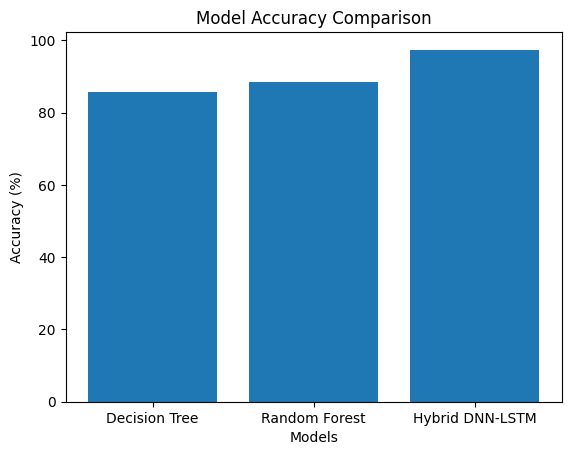
\includegraphics[width=0.5\linewidth]{image.png}
%         \caption{Accuracy comparison of models.}
%         \label{fig:Accuracy}
% \end{figure}



% Moreover, it is evident that, in addition to providing reliable predictions, this technique ensures their quality and reliability, keeping the overall errors in score-related predictions at a minimum, considering several factors that improve the performance of this system.
% This system has evolved beyond the original intention of predicting the outcomes. It is now being utilized as a viable option for the students and the faculty of the department.

% Future Potential and Possible Developments
% In the future, the system has the potential of being more sophisticated and easy to use. This can be done by adding more interpretability so that the users can get an idea of how the prediction is being made, the resume analysis feature can be improved with the latest language processing tools, and the system can be made more applicable for other uses.

% -------------------- REFERENCES --------------------
\begin{thebibliography}{11}

\bibitem{R1}
P.~Cortez and A.~Silva, ``Using data mining to predict secondary school student performance,'' in \textit{Proc. 5th Annu. Future Bus. Technol. Conf.}, EUROSIS, 2008, pp.~5--12.

\bibitem{R2}
E.~A.~Amrieh, T.~Hamtini, and I.~Aljarah, ``Mining educational data to predict student performance using ensemble methods,'' \textit{Int. J. Database Theory Appl.}, vol.~9, no.~8, pp.~119--136, 2016.

\bibitem{R3}
S.~Hussain, N.~B.~Dahan, F.~M.~Ba-Alwi, and N.~Ribata, ``Educational data mining and analysis of students academic performance using WEKA,'' \textit{Indonesian J. Electr. Eng. Comput. Sci.}, vol.~9, no.~2, pp.~447--459, 2018.

\bibitem{R4}
N.~Sghir, A.~Adadi, and M.~Lahmer, ``Recent advances in predictive learning analytics,'' \textit{Educ. Inf. Technol.}, vol.~28, pp.~8299--8333, 2023.

\bibitem{R5}
S.~Hochreiter and J.~Schmidhuber, ``Long short-term memory,'' \textit{Neural Comput.}, vol.~9, no.~8, pp.~1735--1780, 1997.

\bibitem{R6}
F.~Borges, A.~Borges, and A.~Cataldo, ``LSTM-based student performance prediction from LMS activity logs,'' in \textit{Proc. IEEE EDUCON}, IEEE, 2020.

\bibitem{R7}
J.~Xu, K.~H.~Moon, and M.~Van Der Schaar, ``A machine learning approach for tracking and predicting student performance in degree programs,'' \textit{IEEE J. Sel. Topics Signal Process.}, vol.~11, no.~5, pp.~742--753, 2017.

\bibitem{R8}
B.~K.~Bharadwaj and S.~Pal, ``Data mining: A prediction for performance improvement using classification,'' \textit{Int. J. Comput. Sci. Inf. Secur.}, vol.~9, no.~4, pp.~136--140, 2011.

\bibitem{R9}
P.~Chaudhari and A.~Thakkar, ``A survey on student performance prediction in education,'' \textit{Int. J. Comput. Appl.}, vol.~178, no.~7, pp.~1--5, 2019.

\bibitem{R10}
L.~Qiu, Y.~Liu, and X.~Hu, ``Predicting student employability using machine learning,'' \textit{IEEE Access}, vol.~8, pp.~23033--23042, 2020.

\bibitem{R11}
S.~M.~Lundberg and S.~Lee, ``A unified approach to interpreting model predictions,'' in \textit{Proc. Adv. Neural Inf. Process. Syst. (NeurIPS)}, vol.~30, 2017.

\bibitem{R12}
Y.~Zhang, D.~Yeung, and Q.~Xu, ``Probabilistic multi-task learning for activity-independent human motion prediction,'' in \textit{Proc. NIPS}, 2010.

\bibitem{R13}
H.~Chen and H.~Cui, ``Attention-based LSTM for aspect-level sentiment classification,'' in \textit{Proc. EMNLP}, 2016, pp.~606--615.

\bibitem{R14}
T.~Nguyen, S.~Lim, and B.~Le, ``Class imbalance in educational data mining: A survey,'' \textit{Int. J. Educ. Technol. High. Educ.}, vol.~17, no.~1, pp.~1--22, 2020.

\bibitem{R15}
W.~Jiang, Z.~Liu, and Q.~Zheng, ``Combining static and dynamic features for student performance prediction,'' \textit{IEEE Trans. Learn. Technol.}, vol.~14, no.~3, pp.~288--299, 2021.

\bibitem{R16}
D.~P.~Kingma and J.~Ba, ``Adam: A method for stochastic optimization,'' in \textit{Proc. ICLR}, 2015.

\end{thebibliography}
\end{document}
